\documentclass{article}


% load package with some of the available options - you may not need this!
\usepackage[framed,autolinebreaks,useliterate]{mcode}

% for checklist
\usepackage{enumitem,amssymb}
\newlist{todolist}{itemize}{2}
\setlist[todolist]{label=$\square$}
\usepackage{pifont}
\newcommand{\cmark}{\ding{51}}%
\newcommand{\xmark}{\ding{55}}%
\newcommand{\done}{\rlap{$\square$}{\raisebox{2pt}{\large\hspace{1pt}\cmark}}%
\hspace{-2.5pt}}
\newcommand{\wontfix}{\rlap{$\square$}{\large\hspace{1pt}\xmark}}


% something NOT relevant to the usage of the package.
\usepackage{graphicx}
\usepackage{url,textcomp}
\setlength{\parindent}{0pt}
\setlength{\parskip}{18pt}
\title{ECTA Homework 5\\Neuroevolution with the\\Enforced Subpopulations (ESP) algorithm}
\author{\color{blue}Dharmin Bakaraniya, \texttt{dharmin.bakaraniya@smail.inf.h-brs.de}\\
\color{blue}Arun Prabhu, \texttt{arun.prabhu@smail.inf.h-brs.de}}
% //////////////////////////////////////////////////

\begin{document}

\maketitle

\begin{center}
	\begin{minipage}{1\linewidth}
		\begin{center}
			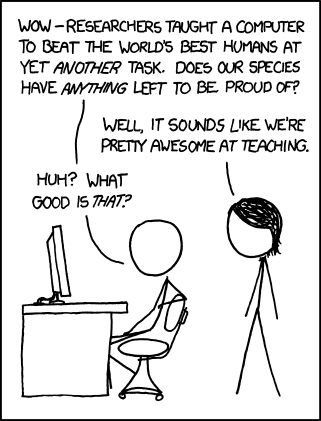
\includegraphics[width=0.7\textwidth]{progeny}
		\end{center}
	\end{minipage}
\end{center}

\newpage

\section{Assignment Description}
	\begin{enumerate}
		\item Solve the following Reinforcement Learning tasks with Neuroevolution.
			\begin{enumerate}
			\item Single Pole Balancing with Velocities
			\item Double Pole Balancing with Velocities
			\item Double Pole Balancing without Velocities
		\end{enumerate}
		\item Compare a standard approach to the ESP algorithm in (c).
	\end{enumerate}

		\begin{itemize}
		\item The task is ``solved'' if the poles does not fall for 1000 time steps.
		\item A 1 and 2 pole balancing simulator function is attached. Given a state and a command it computes the state at the next time step. Examples are included (help: onePole, twoPole). \\\textit{Note:} there is only one 2 pole balancing function, in the case without velocities it is up to you to ``blind'' you ANN of these states, but they are required by the simulator to compute what happens in the next time step.		
		\item You are responsible for all other code, including the ANN.
		\item Additional resources for ESP are available on the LEA
	\end{itemize}

\section{Submission Instructions}
Follow along with the instructions in this PDF, filling in your own code, data, and observations as noted. Your own data should be inserted into the latex code of the PDF and recompiled. All code must be done in MATLAB.

To be perfectly clear we expect two submissions to LEA:
\begin{enumerate}
	\item 1 PDF (report)   -- a modified version of your submission PDF, with your own code snippets, figures, and responses inserted
	\item 1 ZIP (code)     -- a .zip file containing all code use to run experiments (.m files) \textit{and} resulting data as a .mat file
	\item 4 MAT (solution) -- Mat files with the weight matrices of the best found solutions: \textit{spb.mat}, \textit{dpb.mat}, \textit{dpbnv.mat}, and \textit{dpbnv\_esp.mat}
\end{enumerate}





\newpage
\section{The Assignment}

\subsection{Single Pole Balancing (25pts)}
Implement a feed forward network which solves the single pole balancing problem using a fixed topology and a GA or ES (your choice).
\begin{itemize}
	\item (15 pts) Describe your approach. Be sure to mention: the topology of your network, the form of the genotype, the form of the phenotype, the optimization approach used and its details including hyperparameters. Your results should be replicable from your description. Pictures are worth 1000 words.
\color{blue}
\begin{enumerate}
	\item \textbf{Testing with GA} :
	\begin{itemize}
	\item \textbf{Feed Forward Neural Network} was used for this task, to learn the action-reaction behaviour of the environment, using Reinforcement Learning. [Maximum number of steps per episode = 1000]
	\item \textbf{Genotype:} The Genotype represents the weight vector. Each Gene in the Genotype represents the weight of a particular connection of the nodes in the network.Size of Genotype depends on the number of inputs and the neural network topology. The Size of genotype used for the FFN topology mentioned below is given by, \\
    \textit{\textbf{Genotype Size}} = $$(nInput \cdot nHidden) + (nHidden \cdot nOutput)$$ where \\$nInput$:Number of Inputs Nodes\\$nHidden$: Number of Hidden nodes\\$nOutput$: Number of Output Nodes\\
	\textbf{\textit{Genotype Size}} = 4*1 + 1*1 = 5
	\item \textbf{Phenotype:} Phenotype in a way defines the neural network, given that the topology of the network being used is fixed. Phenotype breathes life into a lifeless fixed topology neural network.
	\item \textbf{Optimization Technique:}The tuning of the weights of the Neural Network was done using the Genetic Algorithm. The hyperparameter details are as shown below.
	\begin{enumerate}
	\item \textbf{Population Size:} 10
	\item \textbf{Maximum Generations:} 100
	\item \textbf{Selection Pressure:} 2
	\item \textbf{Crossover Probability:} 0.9
	\item \textbf{Mutation Probability:} 0.4
	\end{enumerate}
	\item \textbf{Feed Forward Neural Network Topology :}
	\begin{enumerate}
	\item Number of Inputs Nodes = 4 = [Cart Position, Cart Velocity, Pole1 Position, Pole1 Angular Velocity]
	\item Number of Hidden Nodes = 1 \textbf{[Only 1 hidden Layer]}
	\item Number of Output Nodes = 1 \textbf{[There is only one output, which is the force to be applied to the cart.]}
	\end{enumerate}
	\end{itemize}
	\item \textbf{Testing with ES} :
	\begin{itemize}
	\item \textbf{Feed Forward Neural Network} was used for this task, to learn the action-reaction behaviour of the environment, using Reinforcement Learning. [Maximum number of steps per episode = 1000]
	\item \textbf{Genotype:} The Genotype represents the weight vector. Each Gene in the Genotype represents the weight of a particular connection of the nodes in the network. Size of Genotype depends on the number of inputs and the neural network topology. The Size of genotype used for the FFN topology mentioned below is given by, \\
    \textit{\textbf{Genotype Size}} = $$(nInput \cdot nHidden) + (nHidden \cdot nOutput)$$ where \\$nInput$:Number of Inputs Nodes\\$nHidden$: Number of Hidden nodes\\$nOutput$: Number of Output Nodes\\
	\textbf{\textit{Genotype Size}} = 4*1 + 1*1 = 5
	\item \textbf{Phenotype:} Phenotype in a way defines the neural network, given that the topology of the network being used is fixed. Phenotype breathes life into a lifeless fixed topology neural network.
	\item \textbf{Optimization Technique:}The tuning of the weights of the Neural Network was done using the basic Evolutionary Strategy. The hyperparameter details are as shown below.
	\begin{enumerate}
	\item \textbf{Population Size:} 1
	\item \textbf{Maximum Generations:} 100
	\item \textbf{Lambda:} 1
	\item \textbf{Sigma:} 1.0
	\item \textbf{Change in Sigma:} 0.5
	\end{enumerate}
	\item \textbf{Feed Forward Neural Network Topology :}
	\begin{enumerate}
	\item Number of Inputs Nodes = 4 = [Cart Position, Cart Velocity, Pole1 Position, Pole1 Angular Velocity]
	\item Number of Hidden Nodes = 1 \textbf{[Only 1 hidden Layer]}
	\item Number of Output Nodes = 1 \textbf{[There is only one output, which is the force to be applied to the cart.]}
	\end{enumerate}
	\end{itemize}
\end{enumerate}
\color{black}
	\item ( 5 pts) Plot the fitness progress over 10 runs.
        \begin{figure}[htpb]
            \centering
            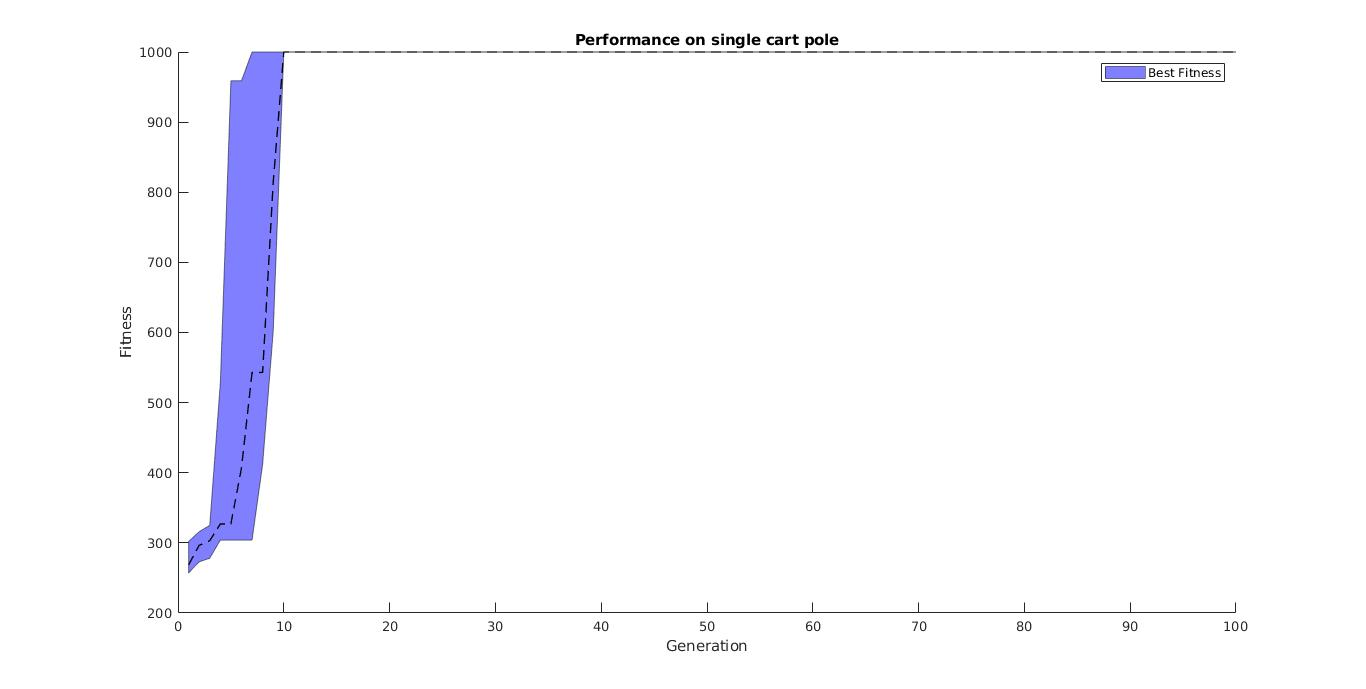
\includegraphics[width=1.0\linewidth]{ga_10exp.jpg}
            \caption{GA Feed forward network for single cart pole balancing problem with above mentioned hyperparameters for 10 experiments}
            \label{fig:}
        \end{figure}
        \begin{figure}[htpb]
            \centering
            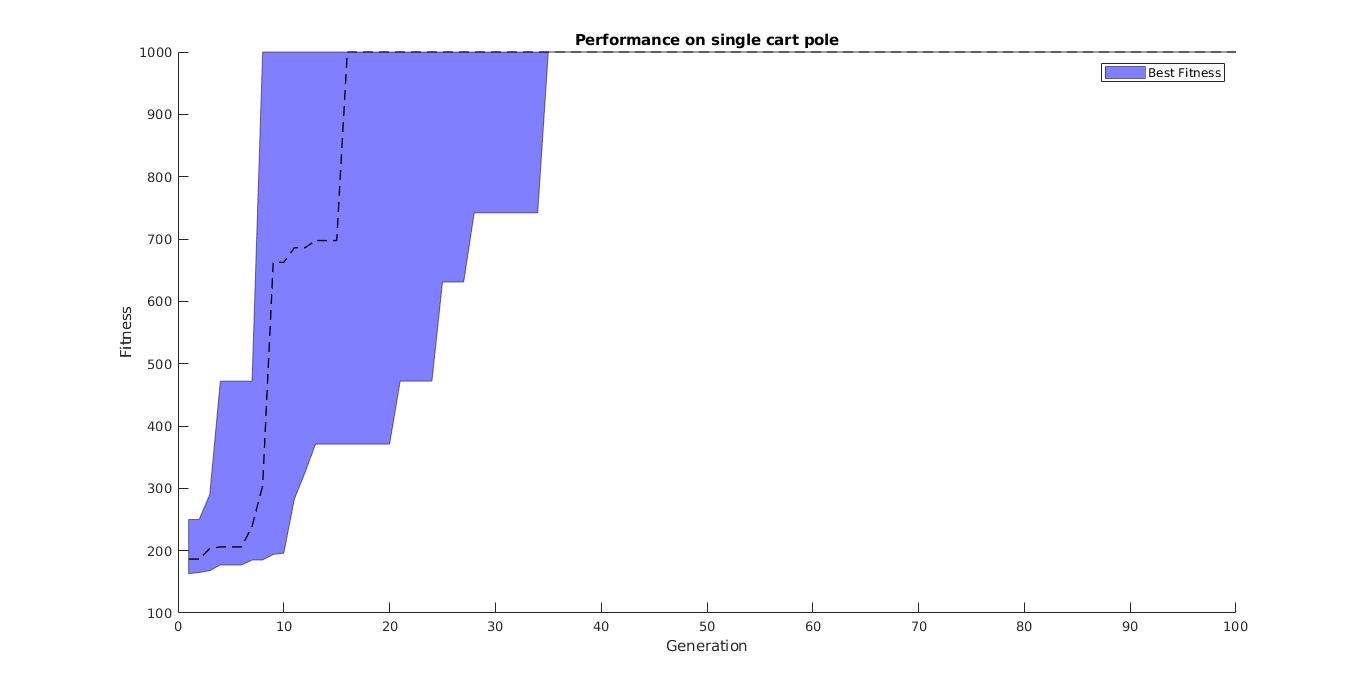
\includegraphics[width=1.0\linewidth]{es_10exp.jpg}
            \caption{ES Feed forward network for single cart pole balancing problem with above mentioned hyperparameters for 10 experiments}
            \label{fig:name}
        \end{figure}
	\item ( 5 pts) Upload the weight matrix of your most successful solution in a file called: \textit{spb.mat}
	\begin{itemize}
	\color{blue}
	\item Out of our solutions using ES and GA, the GA solution performed better and hence the \texttt{spb.mat} represents the GA solution.
	\color{black} 
	\end{itemize}
\end{itemize}

\newpage
\subsection{Double Pole Balancing with Velocities (25pts)}
Adapt your feed forward network to solve the double pole balancing problem.
\begin{itemize}
	\item (15 pts) Describe how this approach differs from above. Your results should be replicable from the this description and the one above.
\color{blue}
\begin{enumerate}
	\item From the above description(ES and GA) almost everything remains the same except the following, irrespective of the optimization technique used (ES or GA).
	\item \textbf{Feed Forward Neural Network Topology :}
	\begin{enumerate}
	\item Number of Inputs Nodes = \color{red}{6 = [Cart Position, Cart Velocity, Pole1 Position, Pole1 Angular Velocity, Pole2 Position, Pole2 Angular Velocity]} \color{blue}
	\item Number of Hidden Nodes = 8 \textbf{[Only 1 hidden Layer]}
	\item Number of Output Nodes = 1 \textbf{[There is only one output, which is the force to be applied to the cart.]}
	\end{enumerate}
	\item \textbf{Genotype :} Size of Genotype depends on the number of inputs and the neural network topology. The Size of genotype used for the FFN topology mentioned below is given by, \\
    \textit{\textbf{Genotype Size}} = $$(nInput \cdot nHidden) + (nHidden \cdot nOutput)$$ where \\$nInput$:Number of Inputs Nodes\\$nHidden$: Number of Hidden nodes\\$nOutput$: Number of Output Nodes\\
	\textbf{\textit{Genotype Size}} = 6*8 + 8*1 = 56
\end{enumerate}
\color{black}	
	\item ( 5 pts) Plot the fitness progress over 10 runs.
        \begin{figure}[htpb]
            \centering
            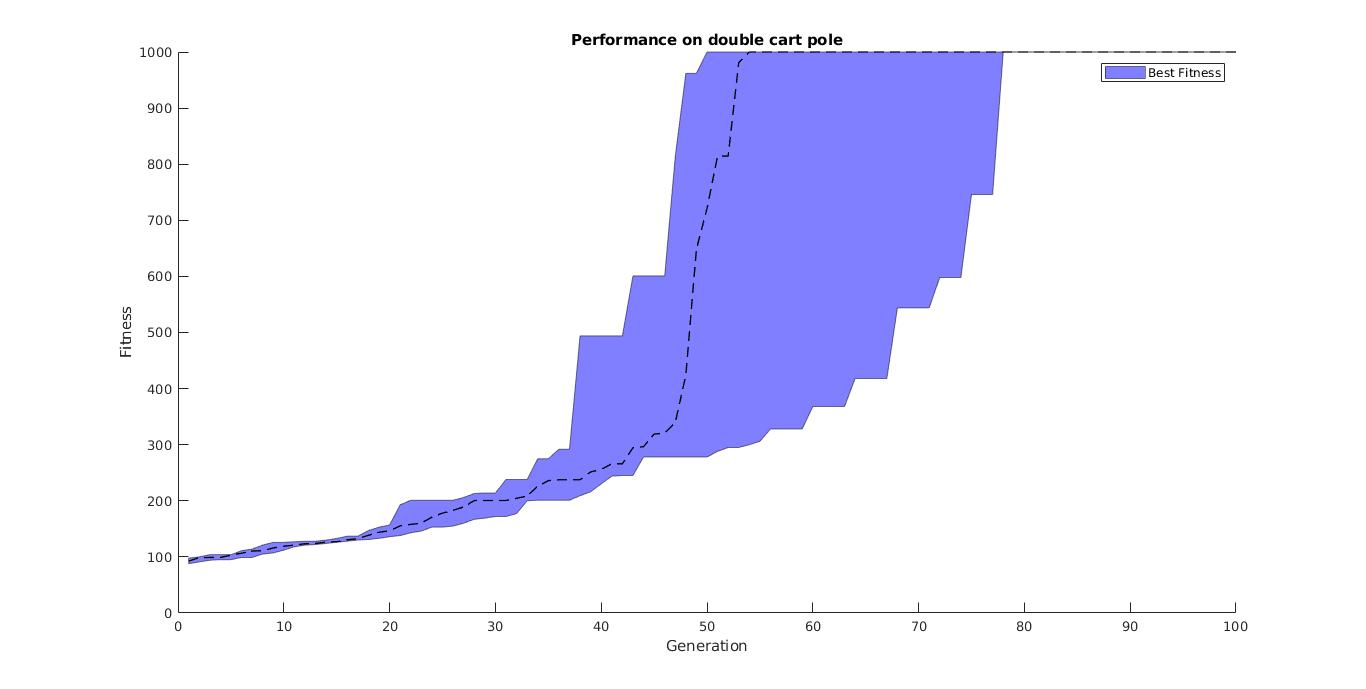
\includegraphics[width=1.0\linewidth]{ga_10exp_2pole.jpg}
            \caption{GA Feed forward network for 2 cart pole balancing problem for 10 experiments with above mentioned hyperparameters}
            \label{fig:}
        \end{figure}
	\item ( 5 pts) Upload the weight matrix of your most successful solution in a file called: \textit{dpb.mat}
	\begin{itemize}
\color{blue}
	\item Out of our solutions using ES and GA, the GA solution performed better and hence the \texttt{dpb.mat} represents the GA solution.
\color{black} 
	\end{itemize}
\end{itemize}

\newpage
\subsection{Double Pole Balancing without Velocities (50pts)}
Alter your network topology to solve the double pole balancing problem without velocities using a recurrent neural network. Implement the ESP algorithm to optimize the same network topology. Compare the performance of the two approaches.
\begin{itemize}
	\item (10 pts) Describe how the first approach differs from above. Your results should be replicable from the this description and the one above.
	\color{blue}
\begin{enumerate}
	\item Recurrent Neural Network is used instead of the Feed Forward Neural Network.
	\item All the entities marked in red are differing from the ones mentioned previously.
	\item \textbf{Recurrent Neural Network Topology :}
	\begin{enumerate}
	\item Number of Inputs Nodes = \color{red}{3 = [Cart Position, Pole1 Position, Pole2 Position]} \color{blue}
	\item Number of Hidden Nodes = 5 \textbf{[Only 1 hidden Layer]}
	\item Number of Output Nodes = 1 \textbf{[There is only one output, which is the force to be applied to the cart.]}
	\end{enumerate}
	\item \textbf{Genotype :} Size of Genotype depends on the number of inputs and the neural network topology also it depends on the type of neural network being used (RNN or FFN). The size of genotype used for the RNN topology mentioned below is given by, \\
    \textit{\textbf{Genotype Size}} = \color{red}$$\big( (nInput+1) \cdot nHidden \big) + \big( nHidden \cdot (nHidden-1) \big)$$ where\\ $nInput$: Number of Inputs Nodes \\$nHidden$: Number of Hidden node\color{blue}\\
	\textbf{\textit{Genotype Size}} = \color{red}(3+1)*5 + 5*4 = 40\color{blue}
\end{enumerate}
\item \textbf{GA related changes:}
\begin{enumerate}
\item \textbf{Population Size:} 10
\item \textbf{Maximum Generations:} \color{red}500\color{blue}
\item \textbf{Selection Pressure:} 2
\item \textbf{Crossover Probability:} 0.9
\item \textbf{Mutation Probability:} \color{red}0.5\color{blue}
\end{enumerate}
\color{black}
	\item (25 pts) Describe the ESP approach, how it differs from above, and other details, including hyperparameters.
	\color{blue}
	\begin{itemize}
	\item \textbf{ESP Approach:}
	Repeat the below steps for a fixed number of Generations.
	\begin{itemize}
	\item \textbf{Initialization:}
	\begin{enumerate}
	\item Number of nodes in the topology is decided.
	\item A sub-population is created for each of the nodes.
	\item Each individual in a sub-population represents a vector of weights, corresponding to the node(to which the sub-population belongs).	
	\end{enumerate}
	\item \textbf{Evaluation:}
	\begin{enumerate}
	\item Select an individual randomly from each subpopulation and create a network from the chosen individuals.
	\item Test the generated network activation on the task and get the fitness of the network.
	\item This fitness value is added to each individuals cumulative fitness.
	\item Repeat this till each individual in each subpopulation has participated in k=5 trials.
	\item Get average fitness of each individual by dividing the cumulative fitness of each individual by number of times that individual participated in the network creation.
	\end{enumerate}
	\item \textbf{Recombination:}
	\begin{enumerate}
	\item Top quartile of each subpopulation is recombined with another individual from same top quartile of that sub population.
	\item The recombined individuals replace the lowest half of the subpopulation.
	  
	\end{enumerate}
	\end{itemize}
	\item \textbf{ESP vs Basic RNN(with GA):}
	\begin{enumerate}
	\item In ESP, the individuals(single node in the network) in each subpopulation are optimized in such a way that when they form the network, the combined network performs well.
	\item In RNN, the the network itself is evolved as a whole, over time rather than evolving each node in the network.
	\end{enumerate}
	\item \textbf{ESP hyperparameters:}
	\begin{enumerate}
	\item \textbf{Sub Population Size:} 10
	\item \textbf{Minimum number of trials per individual} : 5
	\item \textbf{Maximum Generations:} 100
	\item \textbf{Selection Pressure:} 2
	\item \textbf{Crossover Probability:} 1
	\item \textbf{Mutation Probability:} 3/nGenes\\
	where \textbf{nGenes} = (number of inputs + number of hidden nodes) = (3 + 5) = 8 in our case.
 	\end{enumerate}
 	\item Basic RNN hyperparameters(with GA) are as described above.
 	\item The network topology for the ESP is almost same as the one used in the Basic RNN(with GA) described above. Only difference being there is no bias used in ESP.
	\end{itemize}
	\color{black}
	\item (10 pts) Plot the fitness progress of both approaches over 10 runs, including significance
        \begin{figure}[htpb]
            \centering
            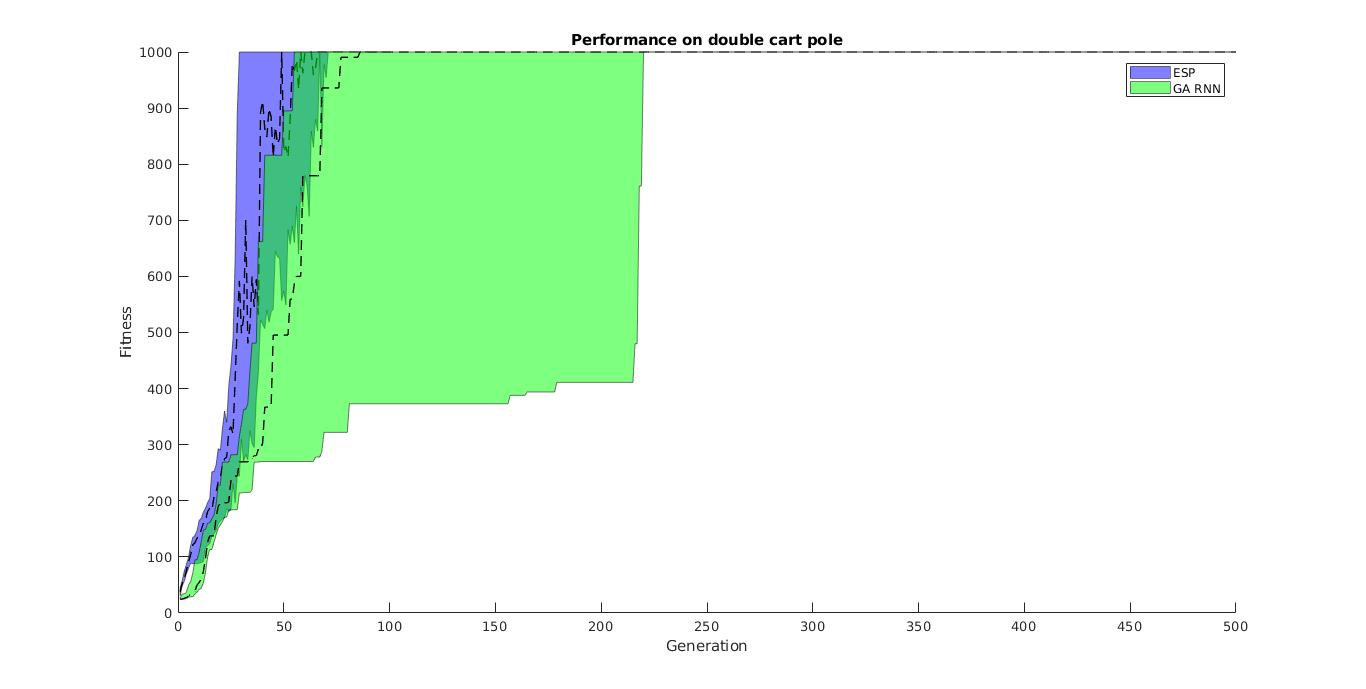
\includegraphics[width=1.0\linewidth]{comparision.jpg}
            \caption{GA RNN vs. ESP for double cart pole balancing problem with above mentioned hyperparameters for 10 experiments. The dotted line represent the median of the best fitness per generation. The area covers by the colored plots are 25 percentile and 75 percentile. The state does not contain velocity information of cart or any of the 2 poles.}
            \label{fig:}
        \end{figure}
	\item ( 5 pts) Upload the weight matrix of your most successful solution in 2 files called: \textit{dpbnv.mat} and \textit{dpbnv\_esp.mat}
        \color{blue}
        The mat file for RNN with GA is provided with \texttt{dpbnv.mat} and ESP weight matrix file is named \texttt{dpbnv_esp.mat}.
        \color{black}
\end{itemize}
\newpage
\section{Coding an ANN in MATLAB}

\end{document}














